\documentclass{patmorin}
\setlength{\parskip}{0mm}
\listfiles
\usepackage{amsthm,amsmath,graphicx,wrapfig}
\usepackage{pat}
\usepackage{paralist}
\usepackage{caption}
%\usepackage{coffee4}
\usepackage[letterpaper]{hyperref}
\usepackage[dvipsnames]{color}
\definecolor{linkblue}{named}{Blue}
\hypersetup{colorlinks=true, linkcolor=linkblue,  anchorcolor=linkblue,
citecolor=linkblue, filecolor=linkblue, menucolor=linkblue, pagecolor=linkblue,
urlcolor=linkblue} 


\usepackage{tikz,hyphenat}
\let\oldmarginpar\marginpar
% renew the \marginpar command to draw 
% a node; it has a default setting which 
% can be overwritten
\renewcommand{\marginpar}[2][rectangle,draw,fill=yellow,rounded corners,text width=2.21cm]{%
        \oldmarginpar{%
        \tikz \node at (0,0) [#1]{#2};}%
        }
\newcommand{\note}[1]{\marginpar{\raggedright\footnotesize\nohyphens{#1}}}

\DeclareMathOperator{\asf}{asf}
\DeclareMathOperator{\xsf}{(a)sf}
\DeclareMathOperator{\strf}{sf}
\DeclareMathOperator{\depth}{depth}
\DeclareMathOperator{\radius}{radius}
\DeclareMathOperator{\msst}{msst}
\newcommand{\mand}{\mathrm{,\,\,and\,}}
\newcommand{\oand}{\mathrm{,\,\,}}
\newcommand{\eps}{\varepsilon}

\title{\MakeUppercase{Average Stretch Factor: How Low Does It Go?}}
\author{Vida Dujmovi\'c, Pat Morin, and Michiel Smid}


\begin{document}
\begin{titlepage}
\maketitle
%\cofeAm{0.7}{0.38}{0}{5.5cm}{3.5in}

\begin{abstract}
  In a geometric graph, $G$, the \emph{stretch factor} between two
  vertices, $u$ and $w$, is the ratio between the Euclidean length of
  the shortest path from $u$ to $w$ in $G$ and the Euclidean distance
  between $u$ and $w$.  The \emph{average stretch factor} of $G$ is
  the average stretch factor taken over all pairs of vertices in $G$.
  We show that, for any constant dimension, $d$, and any set, $V$, of
  $n$ points in $\R^d$, there exists a geometric graph with vertex set
  $V$, that has $O(n)$ edges, and that has average stretch factor $1+
  o_n(1)$.  More precisely, the average stretch factor of this graph is
  $1+O((\log n/n)^{1/(2d+1)})$.  We complement this upper-bound with a
  lower bound: There exist $n$-point sets in $\R^2$ for which any graph
  with $O(n)$ edges has average stretch factor $1+\Omega(1/\sqrt{n})$.
  Bounds of this type are not possible for the more commonly studied
  worst-case stretch factor.  In particular, there exists point sets,
  $V$, such that any graph with worst-case stretch factor $1+o_n(1)$
  has a superlinear number of edges.
\end{abstract}

\end{titlepage}

\section{Introduction}

A \emph{geometric graph} is a simple undirected graph whose vertex set
is a set of points in $\R^d$.  The \emph{average stretch factor} of
a finite connected geometric graph, $G=(V,E)$, with vertex set $V\subset \R^d$
and edge set $E$ is
\begin{equation}
    \asf(G) = \binom{n}{2}^{-1}\sum_{\{u,w\}\in\binom{V}{2}}\frac{\|uw\|_G}{\|uw\|} \eqlabel{asf}
\end{equation}
where $\|uw\|$ denotes the Euclidean distance between $u$ and $w$
and $\|uw\|_G$ denotes the cost of the shortest path from $u$ to $w$
in the graph $G$, where each edge of $G$ is weighted by the Euclidean
distance between its endpoints.  (Here, and forever, $n=|V|$.)

The related notion of \emph{worst-case
stretch factor}, defined as
\[
    \strf(G) = \max_{\{u,w\}\in\binom{V}{2}}\frac{\|uw\|_G}{\|uw\|}  \enspace ,
\]
has been studied extensively.  A graph, $G$, with $\strf(G)\le t$ is
called a \emph{$t$-spanner}.  The construction of and applications
of $t$-spanners is the subject of intensive research and there
is a book \cite{narasimhan.smid:geometric} and handbook chapter
\cite{eppstein:spanning} devoted to the topic.

The average or worst-case stretch factor of the complete graph
with vertex set $V\subset\R^d$ is 1 and, if $V$ contains no
collinear triples, then any graph on $V$ with fewer than $\binom{n}{2}$
edges will have (average and worst-case) stretch factor strictly greater
than 1.  At the other extreme, any connected graph with vertex set $V$
has at least $n-1$ edges.  Thus, there seems to be a tradeoff between
the following two requirements on a graph $G=(V,E)$ that is constructed
from a given point set, $V$:
\begin{compactenum}
  \item $G$ should be as sparse as possible, ideally $|E|\in O(n)$; and

  \item $G$ should have small (average or worst-case) stretch factor,
  ideally $\xsf(G)=1+o_n(1)$.
\end{compactenum}
In this paper we are interested in determining to what extent we can
simultaneously satisfy these two conflicting goals.

For worst-case stretch factor, it is not possible to achieve the preceding
two goals simultaneously: Elkin and Solomon \cite{elkin.solomon:steiner}
show that there exists point sets $V\subset\R^d$ such that any
graph $G=(V,E)$ having $\strf(G)\le 1+\eps$ has maximum degree
$\Omega(1/\eps^{d-1})$.  A variant of their argument shows that,
for some point sets, a constant fraction of vertices must have
degree $\Omega(1/\eps^{d-1})$ and therefore the graph must have
$\Omega(n/\eps^{d-1})$ edges \cite{solomon}. In short: achieving a
worst-case stretch factor of $1+o_n(1)$ requires $\omega(n)$ edges.

%For any $d\in O(1)$ and any $\eps >0$, where $\eps$ may even depend
%on $n$, and any $V\subset\R^d$, $|V|=n$, it is possible to construct
%a graph with $O(n/\eps^{d-1})$ edges such that $\strf(G)\le 1+\eps$
%\cite{carmi.smid:optimal,ruppert.seidel:approximating}.\footnote{We
%note that not all of the classic spanner constructions have an
%optimal dependence on $\eps$ and $d$.  Spanners based on the
%well-separated pair decomposition \cite{callahan.kosaraju:faster}
%can have $\Omega(n/\eps^d)$ edges.} 

%The upper-bound on (worst-case) stretch factor certainly implies the same
%upper-bound for average stretch factor: For any point set, $V$, there
%exists a graph with $\asf(G)=1+\eps$ having $O(n/\eps^{d-1})$ edges.
%Intuitively, though, it should be possible to obtain improved results
%for average stretch factor that, say, reduce the dependence on $\eps$
%and/or $d$.

\subsection{New Results and Outline}

In this paper we show that, for average stretch factor, it \emph{is}
possible to simultaneously achieve both desired properties: For any
constant dimension, $d$, and any set $V\subset \R^d$, there exists
a geometric graph $G=(V,E)$ having $|E|\in O(n)$ edges and such that
$\asf(G)=1+o_n(1)$.  More precisely,
\[
   \asf(G)=1+O((\log n/n)^{1/(2d+1)}) \enspace .
\]
The proof of this result is in \secref{upper-bound} and constitutes the
bulk of the paper.  

In \secref{algorithms}, we show that graphs with small average stretch
factor can be constructed efficiently.  In particular, we present an
$O(n\log n)$ time Monte-Carlo algorithm that, with high probability,
constructs a graph with average stretch factor $1+o_n(1)$.  
In \secref{lower-bound} we present a simple lower-bound that shows our
upper-bound is at least of the right flavour:  For every positive integer
$n$, there exists an $n$ point set in $\R^2$ on which any graph with
$O(n)$ edges has average stretch factor $1+\Omega(1/\sqrt{n})$.
In \secref{discussion} we relate the parts of our construction to some
real-world networks and discuss directions for future work.

\subsection{Relation to Previous Work}

%General results on embedding metric spaces into ultrametrics
%\cite{bartal:graph,fakcharoenphol.rao.ea:tight} imply that, for every set, 
%$V$,  of $n$ points in $\R^d$, there exists a spanning tree, $T=(V,E)$, such
%that $\asf(T)\in O(\log n)$.  

In the more general context of embedding metric spaces into ultrametrics,
Abraham \etal\ \cite{abraham.bartal.ea:metric,abraham.bartal.ea:embedding}
show that for any point set, $V$, there exists a spanning tree,
$T=(V,E)$, with $\asf(T)\in O(1)$.  Thus, it is always possible to
construct a very sparse graph with constant average stretch factor.
This contrasts sharply with worst-case stretch factor: Any spanning
tree on the vertices of a regular $n$-gon has worst-case stretch factor
$\Omega(n)$ \cite[Lemma~15]{eppstein:spanning-report}.

Aldous and Kendall \cite[Section~5.3]{aldous.kendall:short-length}
show that, for any well-distributed\footnote{For example, any
family of point sets that satisfies the quantitative equidistribution
condition \cite[Definition~3]{aldous.kendall:short-length}.} point set
$V\subset[0,\sqrt{n}]^2$ and any $\eps > 0$ there exists a Steiner
network, $N=(V',E)$, with $V'\supseteq V$, of total edge length
$\sum_{uw\in E}\|uw\| \le (1+\eps)\msst(V)$ and for which,
\[
    \binom{n}{2}^{-1}\sum_{\{u,w\}\in \binom{V}{2}}\frac{\|uw\|_N}{\|uw\|} = 1 + O((\log n/n)^{1/3}) .
\]
Here $\msst(V)$ denotes the length of the minimum Steiner spanning tree
of the points in $V$.  Thus $N$ is a graph that is only slightly longer
than the minimum length connected graph that contains $V$ and the average
stretch factor of $N$ (taken over pairs in $V$) tends to 1.  In this
construction, we call the points in $V'\setminus V$ \emph{Steiner points}.

In the work of Aldous and Kendall, which was the starting point for
the current work, the authors focus on finding a \emph{light} network;
one whose total edge length is small.  In the current paper, we focus
instead on finding a \emph{sparse} network; one with a small number
of edges.  With this shift of focus in mind, Aldous and Kendall's
work immediately raises three questions: (1)~Can a similar result be
proven without making any form of ``well-distributed'' assumption on the
points in $V$? (2)~Can a similar result be proven without using Steiner
points? (3)~Can a similar result be proven for point sets in $\R^d$?
Our results answer all three of these questions in the affirmative.

We note that it does not seem easy to answer any of the preceding
questions using a modification of Aldous and Kendall's construction.
(1)~Their proof uses the well-distributed assumption to argue that
most pairs of points are at distance at least $n^{\gamma}$, for any
$\gamma<1/2$ \cite[Section~5.3]{aldous.kendall:short-length}.  (2)~their
construction consists of a minimum Steiner spanning tree of $V$,
some additional random line segments, and some additional segments
that form a grid.  Anywhere two segments cross, a vertex is added
to $V'$, so this construction makes essential use of Steiner points.
(3)~The main technical tool used in their proof is a new result on the
lengths of boundaries of certain cells in arrangements of random lines
\cite[Theorems~3 and 4]{aldous.kendall:short-length}.  In dimensions
greater than 2, arrangements of lines do not decompose space into cells,
so it seems difficult to generalize this result to higher dimensions.

In this extended abstract, we only provide proof sketches.  The full
version of the paper, which has identical numbering of sections,
lemmas, and theorems and differs only in the detail of the proofs,
is included as an appendix and also available as a preprint
\cite{dujmovic.morin.ea:average}.

\section{The Construction}
\seclabel{upper-bound}

Our construction of a good average stretch factor graph, $G=(V,E)$,
makes use of a clustering of the points of $V$ into $O(n/k)$ clusters,
each of size at most $k$, that we call a $k$-partition.  In the next
subsection, we define $k$-partitions and show how to compute them.
In the subsequent subsection we show how to construct the graph $G$.

%The proof that shows the existence of $k$-partitions and especially
%the proof that upper-bounds $\asf(G)$ are sufficiently complicated,
%even without worrying about algorithmic efficiency.  Therefore, we defer
%until the final subsection, a discussion of how to efficiently compute
%the graph $G$.


\subsection{$k$-Partitions}

We make use of the following construct:  A \emph{$k$-partition} of a
set $V$ of $n$ points in $\R^d$ consists of a set, $D$, of balls and an
assignment $f:V\to D$ such that
\begin{compactenum}
  \item $|D|\in O(n/k)$;
  \item for each $u\in V$, $u\in f(u)$ (i.e., $u$ is assigned to a
    ball that contains $u$);
  \item for each $\Delta\in D$, $|\{u\in V: f(u)=\Delta\}|\le k$ (i.e.,
   at most $k$ points are assigned to each ball);
  \item for every $r> 0$ and $p\in\R^d$, the number of balls
   in $D$ whose radius is in the range $[r,2r)$ and that contain $p$
   is $O(1)$; and
  \item for every $r\ge 0$ and every ball, $B$, of radius $r$, 
   \[
      |\{ u\in V : u\in B\text{ and } \radius(f(u))\ge r\}| \in O(k)
   \] 
   (i.e., there are only $O(k)$ points
   of $V$ that are in $B$ and that are assigned to balls of radius at
   least $r$).
\end{compactenum}

Note that, aside from Properties~4 and 5, there is very little structure
to the balls in $D$. In particular, balls in $D$ may overlap and may
even contain each other.  

\begin{lem}\lemlabel{k-partition}
  For any constant dimension, $d$, and any set $V$ of $n$ points in
  $\R^d$, a $k$-partition of $V$ exists and can be computed in $O(n\log
  n)$ time.
\end{lem}

\begin{proof}[Proof Sketch]
  A $k$-partition is constructed by constructing the binary fair-split
  tree, $T$, of the points in $V$ \cite{callahan.kosaraju:decomposition}.
  There is a bijection between the leaves of $T$ and points in $V$, so $T$
  is partitioned, by repeatedly removing a centroid edge, into $O(n/k)$
  subtrees each having at most $k$ leaves.  In this way, each subtree
  defines a single ball $\Delta\in D$ and the leaves of this subtree
  are assigned to the ball $\Delta$.  This establishes Properties~1--3.
  Property~4 is established using a packing argument and known properties
  of fair-split trees \cite[Lemma~9.4.3]{narasimhan.smid:geometric}.
  Property~5 is established using Property~4 and a careful analysis of
  node-to-root paths in fair-split trees.
  %We construct a $k$-partition using the binary \emph{fair-split
  %tree}, $T=T(V)$, which is defined recursively as follows
  %\cite{callahan.kosaraju:decomposition}: If $V$ consists of a single
  %point, $u$, then $T$ contains a single node corresponding to $u$.
  %Otherwise, consider the minimal axis-aligned bounding box, $B(V)$,
  %that contains $V$.  The root of $T$ corresponds to $B(V)$ and this
  %box is split into two boxes $B_1(V)$ and $B_2(V)$ by cutting $B(V)$
  %with a hyperplane in the middle of its longest side.  The left and
  %right subtrees of the root are defined recursively by constructing
  %fair-split trees for $B_1(V)\cap V$ and $B_2(V)\cap V$. See \figref{fst}.
%
  %\begin{figure}
    %\begin{center}
      %\includegraphics{whole-thing}
    %\end{center}
    %\caption{A fair-split tree for $V$ repeatedly splits the bounding
      %box $B(V)$ in the middle of its longest side.}
    %\figlabel{fst}
  %\end{figure}
%
  %\paragraph{The $k$-Partition.}
  %For each node, $u$, of $T$ there is a naturally defined subset
  %$V(u)\subseteq V$ of points associated with $u$ as well as a bounding
  %box $B(u)=B(V(u))$.  Since $T$ is a binary tree with $2n-1$ nodes, it
  %has a set of $t-1$ edges whose removal partitions the vertices of $T$
  %into $t\in O(n/k)$ maximally-connected components $C_1,\ldots,C_t$,
  %each having at most $k$ vertices.
%
  %For each $i\in\{1,\ldots,t\}$, let $u_i$ denote the node in $C_i$ of
  %minimum depth, and call $u_i$, the \emph{root} of $C_i$.
  %To obtain the balls, $\Delta_1,\ldots,\Delta_t$, of the $k$-partition we
  %take, for each $i\in\{1,\ldots,t\}$ the smallest ball, $\Delta_i$ that
  %contains $B(u_i)$.  For the mapping $f$, we map the point associated
  %with each leaf, $w$, of $T$ to the unique ball $\Delta_i$, where $C_i$
  %contains $w$. See \figref{fst-2}.
  %%(Note that a ball, $\Delta_i$,
  %%has no points mapped to it if $C_i$ contains no leaves of $T$; see
  %%\figref{fst-2}.)
%
  %\begin{figure}
    %\begin{center}
      %\includegraphics{whole-thing2}
    %\end{center}
    %\caption{The fair-split tree is partitioned into subtrees of size
    %$k$ (${}=3$) by removing $O(n/k)$ edges.  The root, $u_i$, of each subtree
    %defines a ball, $\Delta_i$, in the $k$-partition. (The ball $\Delta_1$
    %is omitted from this figure.)}
    %\figlabel{fst-2}
  %\end{figure}
%
%
  %The fair-split tree, $T$, and the boxes, $B(u)$, associated
  %with each node, $u$, of $T$ can be computed in $O(n\log n)$ time
  %\cite{callahan.kosaraju:decomposition}.  The partition of the vertices
  %of $T$ into components $C_1,\ldots,C_t$ can easily be done in $O(n\log
  %n)$ time by repeatedly finding an edge of a component of size $k'>k$
  %whose removal partitions that component into two pieces each of size
  %at most $\lceil 2k'/3\rceil$.  Thus, the construction of $D$ and $f$
  %can be accomplished in $O(n\log n)$ time.
%
  %The set of balls $D=\{\Delta_1,\ldots,\Delta_t\}$ and the mapping
  %$f:V\to D$ described in the preceding paragraphs clearly satisfy
  %Properties~1--3 in the definition of a $k$-partition.  What remains
  %is to show that they also satisfy Properties~4 and 5. 
%
  %For a node $u$ in $T$, with $B(u)=[a_1,b_1]\times\cdots\times[a_d,b_d]$,
  %define $L_i(u)=b_i-a_i$ and let $L(u)=\max\{L_i(i):i\in\{1,\ldots,d\}\}$
  %denote the length of $B(u)$'s longest side.   To establish
  %Properties~4 and 5, we make use of the following result on fair-split
  %trees \cite[Lemma~9.4.3]{narasimhan.smid:geometric}:
%
  %\begin{lem}\lemlabel{box-packing}
     %Let $C$ be a box whose longest side has length $\ell$ and let
     %$\alpha >0$ be any positive real number.  Let $w_1,\ldots,w_s$
     %be some nodes of a fair-split tree, $T$, such that
     %\begin{compactenum}
       %%\item $w_i$ is not the root of $T$, for all $i\in\{1,\ldots,s\}$;
       %\item the sets $V(w_i)$ are pairwise disjoint, for all $i\in\{1,\ldots,s\}$;
       %\item $L(w_i)\ge \ell/\alpha$, for all
          %$i\in\{1,\ldots,s\}$;\footnote{The original lemma
          %\cite[Lemma~9.4.3]{narasimhan.smid:geometric} is slightly
          %stronger in that it only requires that $L(w_i')\ge \ell/\alpha$,
          %where $w_i'$ is the parent of $w_i$.} and
       %\item $B(w_i)$ intersects $C$, for all $i\in\{1,\ldots,s\}$.
     %\end{compactenum}
     %Then $s\le (2\alpha + 2)^d$.
  %\end{lem}
  %%Note that the first condition of \lemref{box-packing} is equivalent
  %%to the statement that no $u_i$ is an ancestor of $u_j$ for any
  %%$\{i,j\}\subseteq\{1,\ldots,k\}$, which also implies that the interiors of
  %%$B(u_i)$ and $B(u_j)$ are disjoint.
%
  %\paragraph{Property 4.}
  %To prove that the balls in $D$ satisfy Property~4, let
  %$\{\Delta_{i_1},\ldots,\Delta_{i_q}\}\subseteq D$ be the subset of
  %balls in $D$ having radii in the interval $[r,2r)$ and that all contain
  %some common point, $p\in\R^d$.   Then each such ball, $\Delta_{i_j}$
  %corresponds to a node $u_{i_j}$ of $T$ such that
  %\begin{equation}
        %\frac{2r}{\sqrt{d}} \le L(u_{i_j}) \le 4r \enspace . \eqlabel{bounds}
  %\end{equation}
  %Each box, $B(u_{i_j})$, intersects the ball of radius $2r$ centered at
  %$p$.  (Indeed, the center of $B(u_{i_j})$ is contained in this ball.)
  %Therefore, each box $B(u_{i_j})$ intersects the box, $C$, of side-length
  %$4r$ centered at $p$.
%
  %We are almost ready to apply \lemref{box-packing} to
  %$C$---whose side length is $\ell = 4r$---and the vertex set
  %$w_1,\ldots,w_q=u_{i_1},\ldots,u_{i_q}$. For each $j\in\{1,\ldots,q\}$,
  %$B(u_{i_j})$ intersects $C$, so Condition~3 of \lemref{box-packing}
  %is satisfied.  Furthermore, \eqref{bounds} states that $L(u_{i_j})\ge
  %2r/\sqrt{d} = \ell/(2\sqrt{d})$, so Condition~2 of \lemref{box-packing}
  %is satisfied with $\alpha=2\sqrt{d}$.  Unfortunately, there is still
  %a little more work to do since the nodes $u_{i_1},\ldots,u_{i_t}$
  %do not necessarily satisfy Condition~1 of \lemref{box-packing}.
%
  %To proceed, we partition $u_{i_1},\ldots,u_{i_q}$ into a small number of
  %subsets, each of which satisfies Condition~1 of \lemref{box-packing}.
  %Observe that Condition~1 of \lemref{box-packing} is equivalent
  %to the statement that no $w_i$ is an ancestor of $w_j$ for any
  %$\{i,j\}\subseteq\{1,\ldots,s\}$.  A key observation is that, if $u$
  %is an ancestor of $w$ in a fair-split tree, $T$, and the difference
  %in depth between $u$ and $w$ is at least $d$, then
  %\[
      %L(u) \ge 2L(w) \enspace .
  %\]
  %This, and \eqref{bounds}, implies that, if $u_{i_j}$ is an ancestor
  %of $u_{i_{j'}}$ then
  %\[
     %\depth(u_{i_{j'}})-\depth(u_{i_{j}}) \le d\log(2\sqrt{d}) \enspace .
  %\]
  %Thus, we can partition $u_{i_1},\ldots,u_{i_q}$ into $z=\lceil
  %d\log(2\sqrt{d})\rceil$ subsets, $S_0,\ldots,S_{z-1}$, each of which
  %satisfies Condition~1 of \lemref{box-packing}, by assigning $u_{i_j}$
  %to the subset $S_{\depth(u_{i_j})\bmod z}$.  
%
  %Now, \lemref{box-packing} implies that, for each $i\in\{0,\ldots,z-1\}$, 
  %\[
     %|S_i|\le (4\sqrt{d}+2)^d
  %\]
  %so that
  %\[
     %q = \sum_{i=0}^{z-1}|S_i|\le (4\sqrt{d}+2)^dz 
       %= (4\sqrt{d}+2)^d\lceil d\log(2\sqrt{d})\rceil  
       %\in O(1) \enspace .
  %\]
  %Thus, for any point $p\in\R^d$, the set of balls in $D$ whose radius
  %is in the interval $[r,2r)$ and that contain $p$ has size $O(1)$.
  %Therefore the balls in $D=\{\Delta_1,\ldots,\Delta_t\}$ satisfy
  %Property~4 in the definition of a $k$-partition.
%
  %\paragraph{Property 5.}
  %To study Property~5, it is easier to work with the bounding boxes,
  %$B(u)$, associated with each node, $u$, in the fair-split tree as
  %well as the box, $C$, of side length $2r$ that contains the ball $B$.
  %See \figref{property-5}.  Observe that if some ball, $\Delta_i$,
  %is assigned a point in $B$, then the box $B(u_i)$ intersects $C$.
  %Thus, we need only consider the set $U\subseteq\{u_1,\ldots,u_t\}$
  %that contains only those nodes $u_i$ such that $\radius(\Delta_i)\ge r$
  %and $B(u_i)$ intersects $C$.
%
  %\begin{figure}
    %\begin{center}
      %\includegraphics{property-5}
    %\end{center}
    %\caption{Proving Property~5 of $k$-partitions.}
    %\figlabel{property-5}
  %\end{figure}
%
  %For each $u\in U$, \eqref{bounds} implies that $L(u)\ge 2r/\sqrt{d}$.
  %Therefore, by \lemref{box-packing}, $U$ contains a subset, $U'$, of
  %size at most $(4\sqrt{d}+2)^d\in O(1)$ such that every node in $U$
  %is an ancestor of some node in $U'$.  Thus, the elements of $U$ can be
  %covered by $O(1)$ paths, each of which goes from a node in $U'$ to the 
  %root of $T$.  It suffices to consider the contribution of one such
  %path, $w_1,\ldots,w_\ell$, where $w_1\in U'$ and $w_\ell$ is the root
  %of $T$.
%
  %For each $i\in\{1,\ldots,\ell\}$, let $C_{i}$, denote the box $C\cap
  %B(w_{i})$.  Since $B(w_1)\subset\cdots\subset B(w_\ell)$, we have that
  %$C_1\subseteq\cdots\subseteq C_\ell$. Observe that, for each $w_i$, the
  %ball associated with $w_i$ is not assigned any points in $B(w_{i-1})$.
  %Thus, it is sufficient to show that there are $O(1)$ values of $i$
  %for which $V\cap C_i\neq V\cap C_{i-1}$; for each such $i$, the number
  %of elements assigned to the corresponding ball of the $k$-partition
  %is at most $k$.
%
  %We extend the side-length notation, $L_i$, to any box,
  %$B=[a_1,b_1]\times\cdots[a_d,b_d]$, so that $L_i(B)=|b_i-a_i|$ and
  %define the \emph{total side length} $\sum_{i=1}^d L_i(B)$.  We will
  %show that, for each $i\in\{2,\ldots,\ell\}$, at least one of the
  %following statements is true
  %\begin{compactenum}
    %\item $V\cap C_i = V\cap C_{i-1}$; 
    %\item the total side length of $C_i$ exceeds that of $C_{i-1}$ by at least
      %$L(w_1)/2$; or
    %\item $C_i$ intersects a side of $C$ that is not intersected by $C_{i-1}$.
  %\end{compactenum}
  %This is sufficient to prove the result since Case~1 does not result in
  %any new points included in $B$, Case~2 can occur at most $4rd/L(w_1)\in
  %O(1)$ times, and Case~3 can occur at most $2d\in O(1)$ times.
%
  %To see why one of the preceding cases must occur, suppose that neither
  %Case~1 nor Case~3 applies.  Since Case~1 does not apply, there is
  %some point $q\in V\cap C_i$ that is not in $C_{i-1}$. 
  %Without loss of generality, assume that the fair-split tree cuts
  %$B(w_i)$ with a plane, $\Pi$, that is perpendicular to the $x_1$-axis.
  %Let $\Pi^+$ and $\Pi^-$ denote the closed halfspaces bounded by $\Pi$
  %that contain $q$ and $B(w_{i-1})$, respectively.  Then we have that
  %\[
      %L_1(B(w_i)\cap \Pi^+) 
          %= L_1(w_i)/2 
          %\ge L(w_{i-1})/2 
          %\ge L(w_{1})/2  \enspace .
  %\]
  %Observe that $B(w_{i})$ does not intersect the side of $C$ that is
  %parallel to $\Pi$ and contained in $\Pi^+$ (since, otherwise, Case~3
  %would apply).  This implies that
  %\[
      %L_1(C_i) \ge L_1(C_{i-1}) + L(w_1)/2 \enspace .
  %\] 
  %Thus, if neither Case~1 nor Case~3 applies to $u_i$, then Case~2
  %applies.  This completes the proof.
\end{proof}

\subsection{The Graph $G$}

With the availability of $k$-partitions, we are now ready to construct
a graph $G$ with low average stretch factor.  In the following construction,
positive valued variables $c,k\in\omega_n(1)$ and $\epsilon\in o_n(1)$
are used without being specified.  Values of these variables that
optimize the average stretch factor of $G$ will be given in the proof
of \thmref{upper-bound}.  In the meantime, the reader can mentally assign the
values $c=k=\log n$ and $\epsilon = 1/\log n$, which are sufficient to
prove that $\asf(G)=1+o_n(1)$.

\paragraph{Hubs.}

We begin with a $k$-partition $(\{\Delta_1,\ldots,\Delta_{n'}\},f)$
of $V$.  For each $i\in\{1,\ldots,n'\}$, let $r_i$ denote the radius of
$\Delta_i$.  We will use the convention that $\Delta_1,\ldots,\Delta_{n'}$
are ordered by increasing radii, so that $r_i \le r_j$ for each $1\le
i < j\le n'$.  For each $i\in \{1,\ldots,n'\}$, let $V_i=\{u\in V :
f(u)=\Delta_i\}$; that is, $V_i$ is the set of points assigned to the
ball $\Delta_i$.  For each set $V_i$, we choose a \emph{hub}, $u_i\in
V_i$, arbitrarily. Let $H=\{u_1,\ldots,u_{n'}\}$ denote the set of hubs
and recall that $|H|=n'\in O(n/k)$.

\begin{figure}
  \begin{minipage}{.47\textwidth}
    \centering{\includegraphics[width=.95\linewidth]{hitter}}
    \captionof{figure}{The ball $E_i$ captures as many points of $V$ as possible
     while still intersecting $D_i$.}
    \figlabel{hitter}
  \end{minipage}%
  \hspace{.06\textwidth}
  \begin{minipage}{.47\textwidth}
      \centering{\includegraphics[width=.95\linewidth]{overview}}
    \captionof{figure}{$G$ contains a 2-spanner of $V$ (gray edges) as well as
      $O(n/k)$ hubs whose centers are interconnected by a
      $(1+1/k^{1/(d-1)})$-spanner (red edges)}
    \figlabel{overview}
  \end{minipage}
\end{figure}

\paragraph{Roads and Highways.}

Our graph $G$ starts with two spanner constructions.
The first spanner (the roads) is denoted by
$G_2=(V,E_2)$, is a 2-spanner of $V$, and has $O(n)$ edges
\cite{callahan.kosaraju:faster,salowe:constructing,vaidya:sparse}.
The next spanner (the highways) is denoted by $G_1=(H,E_1)$, is a
$(1+1/k^{1/(d-1)})$-spanner of $H$, and has $O(k|H|)=O(n)$ edges
\cite{carmi.smid:optimal,ruppert.seidel:approximating}.

With $G_1$ and $G_2$ we have, for any $u,w\in V$:
\[
   \frac{\|uw\|_G}{\|uw\|} \le \begin{cases}
         1+1/k^{1/(d-1)} & \text{if $u,w\in H$ (by using $G_1$)} \\
         2 & \text{in any case (by using $G_2$).}
       \end{cases}
\]

\paragraph{Covering a Nearby Cluster.}

Informally, the idea behind the graphs $G_1$ and $G_2$ is that, if
$u\in V_i$ and $w\in V_j$ are ``far apart'' (relative to $r_i$
and $r_j$), then the path from $u$ to $w$ that goes from $u$ to $u_i$
via roads ($G_2$), then to $u_j$ via highways ($G_1$), and then onto
$w$ via roads again should have length $(1+o_n(1))\|uw\|$.  Of course,
this only works if $u$ and $w$ are far apart.  The final step of
our construction attempts to deal with the majority of cases where $u$
and $w$ are not far apart.

To make the preceding ideas precise, Let $r_i$ denote the radius
of $\Delta_i$ and let $D_i$ be the ball centered at the center of
$\Delta_i$ and having radius $cr_i$.  Points of $V$ that are in $D_i$
can be problematic for $V_i$; there is no guarantee that such points
have paths with $1+o_n(1)$ stretch factor to the points in $V_i$.

For each $i\in\{1,\ldots,n'\}$, we find a ball, $E_i$, of radius $r_i/c$,
that intersects $D_i$, and that contains the maximum number of points
of $V$.  (Note that this may include points of $V$ in $V_i$ or outside
of $D_i$.)  We then add edges joining each of the points in $V_i$ to
a carefully chosen point $w_i\in E_i$.  See \figref{hitter}.

The point $w_i$ is chosen as follows: For each point $w\in V$, let
$i(w)\in \{1,\ldots,n'\}$ denote the smallest index such that $w\in
E_{i(w)}$ and $|E_{i(w)}\cap V| \ge \epsilon n$; if no such index exists,
let $i(w)=\infty$.  The point $w_i\in E_i$ is selected to be any of the
points in $E_i$ that minimizes $i(w)$.  This concludes the description
of the graph $G$.


\subsection{Two Illustrative Examples}
Before delving into the proof that $G$ has low average stretch factor,
it may be helpful to study two examples that illustrate why the balls
$E_1,\ldots,E_{n'}$ are needed and why the choice of the representative
vertices, $w_i\in E_i$, is  important.

\paragraph{Example 1: Exponential Grids.}
The first example is a set of points arranged as a sequence of
$\sqrt{k}\times\sqrt{k}$ grids, $G_0,\ldots,G_{n/k-1}$.  The grid $G_i$
has its center on the x-axis at x-coordinate $2^{i+1}-1$, and has side
length $2^i$ (see \figref{grid}). The natural $k$-partition of this
grid is the one that assigns all points in each $G_i$ to a single ball,
$\Delta_i$.  In this grid, if we consider $G_i$, for some large value
of $i$, we see that all the points in $G_0,\ldots,G_{i-1}$ are within
distance $O(2^{i})$ of all the points in $G_i$.  Forcing every path from
every $u\in G_i$ to every $w\in G_{j}$, $j<i$, to go through a central
vertex $u_i\in G_i$ would be too costly; on average the detour through
$u_i$ would increase the length of this path by $\Omega(2^{i})$.

\begin{figure}
  \begin{minipage}{.47\textwidth}
    \centering{\includegraphics[width=.9\linewidth]{grids}}
    \captionof{figure}{A sequence of exponentially increasing grids
       illustrates the need for connecting all points in $V_i$ to some
       point in $E_i$.}
    \figlabel{grid}
  \end{minipage}
  \hspace{.06\textwidth}
  \begin{minipage}{.47\textwidth}
    \centering{\includegraphics[width=.95\linewidth]{example2}}
    \captionof{figure}{An illustration of why it is important to choose
      $w_i$ carefully.  A bad choice (like the one illustrated) leads to
      a significant detour on the paths from every $u\in V_i$ to every
      $w\in E_j$.}
    \figlabel{example2}
  \end{minipage}
\end{figure}

The ball $E_i$ solves the preceding problem; $E_i$ is large enough
to cover all points in $G_0,\ldots,G_{i-\Theta(\log c)}$.  The path
from $u\in G_i$ directly to $w_i\in E_i$ and then to any $w\in E_i$
has length at most
\[
    \|uw\| + O(2^{i}/c) \enspace .
\]
Furthermore, all of the points in $E_i$ are at distance $\Omega(2^i)$ from
all the points in $G_i$, so $\|uw\|_G/\|uw\| = 1+O(1/c)$.  Part~3 of the
proof of \thmref{upper-bound} is dedicated to showing that, in general,
the balls $E_1,\ldots,E_{n'}$ help with many pairs of points that would
otherwise be problematic.
\paragraph{Example 2: The Importance of Choosing Wisely.}
Our second example is intended to illustrate the importance of carefully
choosing the representative vertex $w_i\in E_i$.   In this example, there
is a dense cluster of $n/2$ points that is contained in some ball $E_j$
(see \figref{example2}).  Consider now some $i>j$ such that $r_i$ is
much greater than $r_j$.  It is easy to make a configuration of points so
that, for some cluster $V_i$, the corresponding ball $E_i$ contains $E_j$
as well as a few other points that are far from $E_j$. If one of these
points is used as the representative vertex, $w_i$, then all $kn/2$ paths
from $u$ in $V_i$ to $w\in E_j$ will have to make a detour through $w_i$.
By repeating this for many different values of $i$, this is enough to
produce an average stretch factor significantly larger than 1.

The choice of $w_i$ is designed to avoid the preceding problem.  In this
example, $w_i$ would be chosen from the points in $E_j$, since $r_j <
r_i$ and $E_i$ contains $n/2\ge \epsilon n$ points of $V$.  Part~4 of
the proof of \thmref{upper-bound} is dedicated to showing this careful
choice of $w_i$ works.  In particular, it ensures that, for most pairs
of the form $u\in V_i$, $w\in E_i$,
\[
    \|uw_i\| + O(\|w_iw\|) = \|uw\|(1+O(1/c)) \enspace .
\]

%\begin{wrapfigure}[16]{r}{.5\linewidth}
%  \begin{center}
%    \includegraphics[width=.95\linewidth]{example2}
%  \end{center}
%  \caption{An illustration of why it is important to choose $w_i$ carefully.
%    A bad choice (like the one illustrated) leads to a significant detour
%    on the paths from every $u\in V_i$ to every $w\in E_j$.}
%  \figlabel{example2}
%\end{wrapfigure}



\subsection{The Proof}

Without further ado, we now prove that $G$ has low average stretch factor.

\begin{thm}\thmlabel{upper-bound}
  For every constant dimension, $d$, and every set, $V$, of
  $n<\infty$ points in $\R^d$, the graph $G=(V,E)$ described above
  has $O(n)$ edges and $\asf(G)=1+o_n(1)$.  More precisely,
  $\asf(G)=1+O((\log n/n)^{1/(2d+1)})$.
  % there exists a geometric graph $G$ with
  % $V(G)=V$, $|E(G)|\in O(n)$ and $\asf(G)=1+o_n(1)$. 
  % More precisely, $\asf(G)=1+O((\log n/n)^{1/2d})$.
\end{thm}

\begin{proof}
  That $G$ has $O(n)$ edges follows immediately from its definition.

  To upper-bound the average stretch factor of $G$, there are four types
  of pairs of points, $u\in V_i$, $w\in V_j$, $j\ge i$, to consider
  (recall that $\Delta_1,\ldots,\Delta_{n'}$ are ordered so that $r_i \ge r_j)$:
  \begin{compactenum}
    \item pairs that are both from the same set, i.e., where $i=j$;
    \item pairs for which $w$ is outside of $D_i$;
    \item pairs for which $w$ is contained in $D_i\setminus E_i$; and
    \item pairs for which $w$ is contained in $E_i\cap D_i$.
  \end{compactenum}
  We consider each of these types of pairs in turn.  Our strategy is to
  study the $\binom{n}{2}$ terms that define $\asf(G)$ in \eqref{asf}.
  We will show that $o(n^2)$ of these terms are at most 2 while the
  remaining terms are at most $1+o_n(1)$.  Thus,
  \[
     \asf(G)\le \binom{n}{2}^{-1}\left(2\cdot o(n^2)
                                       +\binom{n}{2}(1+o_n(1))\right)
     = 1+o_n(1) \enspace .
  \]

  \paragraph{Type~1 Pairs.}
  Each $V_i$, for $i\in\{1,\ldots,n'\}$, defines at most $\binom{k}{2}$
  Type~1 pairs, so the total number of Type~1 pairs that contribute a
  term to the sum in \eqref{asf} is at most
  \[
    \binom{k}{2}\cdot O(n/k) \in O(nk)
      \enspace .
  \]

  \paragraph{Type~2 Pairs.}
  For each Type~2 pair $u\in V_i$, $w\in V\setminus D_i$, there is a
  path from $u$ to $u_i$ in $G_2$, then from $u_i$ to $u_j$ in $G_1$
  and then finally from $u_j$ to $w$ in $G_2$ whose length is at most
  \[
     4r_i + \|u_iu_j\|_G + 4r_j
      \le (1+1/k^{1/(d-1)})(\|uw\| + 16r_i) \enspace .
  \]
  Furthermore, $\|uw\|\ge (c-1)r_i$ since $w$ is outside of $D_i$.
  Therefore, for each Type~2 pair, the term that appears in \eqref{asf}
  is of the form
  \[
    \frac{\|uw\|_G}{\|uw\|}\le (1+1/k^{1/(d-1)})(1+O(1/c)) 
       = 1+O(1/k^{1/(d-1)}+1/c) \enspace .
  \]

  \paragraph{Type~3 Pairs.} Using Property~4 of $k$-partitions and the
  fact that $E_i$ is chosen to maximize the number of points it contains,
  it is possible to show that the number of terms in \eqref{asf} contributed
  by Type~3 pairs is $O\left(\sqrt{kn^3c^d\log c}\right)$.

  \paragraph{Type~4 Pairs.}  Using Property~5 of $k$-partitions, and the
  special choice of $w_i\in E_i$, it is possible to show that the number
  of Type~4 pairs that contribute more than $O(1/c)$ to \eqref{asf}
  is at most $O(\epsilon n^2)$.

  \paragraph{Finishing Up.}
  Putting together the contributions of all four types of pairs, we obtain
  \begin{equation}\eqlabel{master-asf}
     \asf(G) = 1 + O\left(1/k^{1/(d-1)} + 1/c 
       + \binom{n}{2}^{-1}\left(kn+\sqrt{kn^{3}c^{d}\log c}
             +\epsilon n^2\right)\right) \enspace .
  \end{equation}
  Optimizing over $\epsilon$, $k$, and $c$, yields
  \[
     \asf(G) = 1+ O\left(\left(\frac{\log n}{n}\right)^{1/(2d+1)}\right) \enspace . \qedhere
  \]
\end{proof}

%\begin{rem}\remlabel{epsilon-choice}
%   In the next section, efficient algorithms will require that
%   $\epsilon = (\log^\kappa n)/k$ for some constant $\kappa \ge 0$.
%   Since the bound on the average stretch factor requires that
%   $\epsilon\in\Omega((k/n)^{1/3})$, this implies that the value of $k$
%   must be at most $n^{1/4}$.  The following table shows the optimal
%   choices of $k$ and $c$ for different dimensions, $d$:
%
%   \begin{center}
%   \renewcommand\arraystretch{1.3} %\setlength\minrowclearance{2.4pt}
%     \begin{tabular}{|r|l|l|l|}
%        \hline
%        $d$ & $k$ & $c$ & $\asf(G)$ \\\hline\hline
%        $2$ & $(n/\log n)^{1/5}$ & $(n/\log n)^{1/5}$ 
%              & $1+ O((\log^{5\kappa+1} n/n)^{1/5})$ \\
%        $\ge 3$ & $n^{1/4}$ & $(\log n/n^{3/4})^{1/(d+2)}$ 
%              & $1+ O(1/n^{1/(4d-4)})$ \\
%     \hline
%     \end{tabular}
%   \end{center}
%\end{rem}

\section{Algorithms}
\seclabel{algorithms}

In this section, we discuss efficient algorithms for computing a graph
$G=(V,E)$ that has low average stretch factor, given the point set
$V\subset\R^d$.  We first present a fairly straightforward adaptation of
the construction given in the preceding section that yields an $O(n\log^d
n)$ time algorithm.  We then show that some refinements of this algorithm
lead to an $O(n\log n)$ time algorithm.

Our algorithms are randomized.  Throughout this section, we say that an
event within an algorithm happens \emph{with high probability} if the
event occurs with probability at least $1-O(n^{\alpha})$ and $\alpha$
can be made into an arbitrarily large constant by increasing the running
time of the algorithm by a constant factor.

\subsection{A Simple Algorithm}

For ease of exposition, we start with a simple algorithm that is
relatively faithful to the proof of \thmref{upper-bound}.  
\begin{thm}\thmlabel{algorithm}
  For every constant dimension, $d$, and every set, $V$, of $n<\infty$
  points in $\R^d$, there exists a randomized $O(n\log^{d} n )$ time
  algorithm that constructs a graph $G'=(V,E)$ that has $O(n)$ edges and,
  with high probability, 
  \[
      \asf(G')=\begin{cases}
         1+ O((\log n/n)^{1/5}) & \text{for $d=2$} \\
         1+ O(1/n^{1/(4d-4)}) & \text{for $d\ge 3$} \\
      \end{cases}
  \]
\end{thm}


\begin{proof}
  Throughout this proof, a \emph{box} is an axis-aligned box of the form
  $[a_1,b_1]\times\cdots\times[a_d,b_d]$ and we call this a \emph{square
  box} if $b_i-a_i=b_j-a_j$ for all $i,j\in\{1,\ldots,d\}$. For a box,
  $B$, let $L(B)$ denotes the length of the longest side of the box, $B$.
  The graph $G'$ constructed by our algorithm is similar to the graph,
  $G$, described in the previous section, except for three major
  differences:
  \begin{compactenum}
     \item Every element in $G$ that is defined in terms of a ball is
     now defined in terms of a square box.  In particular,
     \begin{compactenum}
       \item $\Delta_1,\ldots,\Delta_{n'}$ are minimal square boxes that contain
         the corresponding boxes defined by nodes of the fair-split tree;
       \item $D_1,\ldots,D_{n'}$ are square boxes where each $D_i$
         is a square box of side-length $cL(\Delta_i)$ centered at the
         center of $\Delta_i$; and
       \item $E_1,\ldots,E_{n'}$ are square boxes where each $E_i$ is a box of
         side-length $L(\Delta_i)/c$ that intersects $D_i$.
     \end{compactenum}
     \item The box $E_i$ does not perfectly maximize the number of points
       it contains. Instead, we guarantee that, if there exists any
       box of side-length $L(\Delta_i)/2c$ that intersects $D_i$ and
       contains $m\ge \epsilon n$ points of $V$, then $E_i$ is chosen so that
       it contains at least $m$ points of $V$.
     \item We change the value of $\epsilon$ to $\epsilon = 1/k$
      and use slightly different values of $c$ and $k$.
  \end{compactenum} 
  It is straightforward, but tedious, to check that the proof of
  \thmref{upper-bound} using these new definitions of $\Delta_i$, $D_i$,
  and $E_i$ shows that the graph $G'$ satisfies the requirements of the
  theorem.  To construct $G'$ in $O(n\log^d n)$ we make extensive use
  of range trees \cite{bentley:multidimensional,luecker:data} at each
  step as well as random sampling to find the boxes $E_1,\ldots,E_{n'}$.
\end{proof}

\subsection{A Faster Algorithm}

In the preceding section we gave an $O(n\log^d n)$ time algorithm.
In this section, we show that the running time can be reduced to $O(n\log
n)$ with only a small increase in the average stretch factor.

\begin{thm}\thmlabel{algorithm-faster}
  For every constant dimension, $d$, and every set, $V$, of $n<\infty$
  points in $\R^d$, there exists a randomized $O(n\log n)$ time
  algorithm that constructs a graph $G''=(V,E)$ that has $O(n)$ edges
  and, with high probability, 
  \[
      \asf(G'')=\begin{cases}
         1+ O((\log^{6} n/n)^{1/5}) & \text{for $d=2$} \\
         1+ O(\log^{(d-2)/(d-1)}n/n^{1/(4d-4)}) 
                  & \text{for $d\ge 3$} 
      \end{cases}
  \]
\end{thm}

\begin{proof}[Proof Sketch]
  The construction of $G''$ is similar to the construction of $G'$
  described in the proof of \thmref{algorithm} but makes more extensive
  use of random sampling so that the range trees it uses contain only
  $O(n/\log^d n)$ points and only $O(n/\log^d n)$ queries are performed on
  these trees.
\end{proof}



\section{Lower Bounds}
\seclabel{lower-bound}

Next, we prove a simple lower-bound which shows that our bound on the
average stretch factor is at least of the right flavour: Combined with
the upper-bound of \thmref{upper-bound}, the following result shows that
the optimal bound is $1+O(1/n^{\delta})$ for some $\delta\in(1/(2d+1),1/2]$.

\begin{thm}\thmlabel{lower-bound}
  For every positive integer, $n$, there exists a set, $V$, of $n$
  points in $\R^2$, such that every geometric graph, $G$, with vertex
  set $V$ and having $O(n)$ edges has $\asf(G)\ge 1 + \Omega(1/\sqrt{n})$.
\end{thm}

\begin{proof}[Proof Sketch]
  An easy analysis where $V$ consists of $n$ points evenly spaced on
  opposite sides of a square establishes this lower bound.
\end{proof}

We remark that the proof of \thmref{lower-bound} is easily modified to
provide a tradeoff between the number of edges of $G$ and the average
stretch factor.  In particular, if $G$ has $m\in o(n^2)$ edges, then
\[
   \asf(G) \ge 1 + \Omega(1/\sqrt{m}) \enspace .
\]

\section{Discussion}
\seclabel{discussion}

We have shown that, for any set, $V$, of $n$ points in $\R^d$, we can
construct, in $O(n\log n)$ time, a graph on $V$ whose average stretch
factor is $1+o_n(1)$.  Our construction consists of three parts, (1)~a
2-spanner, $G_2$ of $V$, (2)~a $1+o_n(1)$-spanner of a subset $H\subset V$
of so-called hubs, and (3)~a collection of edges that join all vertices
within each group, $V_i$, to a single representative vertex, $w_i$,
within a very dense (compared to $V_i$) set of vertices, $E_i\cap V$.

\subsection{Realistic Networks(?)}

We note that, if one has some form of reasonable well-distributed
assumption about the points in $V$, like that used by Aldous and Kendall,
then it is fairly straightforward to show that the first two parts of
our construction are sufficient to obtain an average stretch factor
of $1+o_n(1)$. The third part of our construction is only required
to deal with instances in which there are exponential differences in
density of points of $V$.  It seems natural to ask whether this part
of the construction is necessary in any real-world network or whether
the vertices of real-world networks are always well-distributed.

The first two parts of our construction are quite natural and can be
recognized in many real-world networks.  The most common (though admittedly,
imperfect) example is road networks where individual buildings are
interconnected by roads, which very often form a partial grid (a
$\sqrt{2}$-spanner). The cities, towns, and villages, containing these
buildings are themselves interconnected by a relatively fast, and fairly
direct, system of highways.

The third part of our construction seems less natural.  In road networks,
this part of the construction would correspond to densely-populated
areas that have several direct routes to them from well-separated
locations.  Since this part of our construction is only required to
deal with pathological cases involving inter-point distances that vary
exponentially, one might think that it does not appear in real-world
networks.

A quick inspection of the U.S. Highway System shows that, even by 1926,
there were many direct highway connections to Chicago, Detroit, Kansas
City, Memphis, Newport, and other large cities (see \figref{us-map}).
These highways were expensive and would have been built unless they
added real value to the road network.  While this does not correspond
perfectly with the third part of our construction, it does suggest that
a simple two-level network of clusters, each having a single hub, does
not produce real-world networks of sufficient quality; \emph{some}
form of extra augmentation is necessary.

\begin{figure}
  \begin{tabular}{@{}c@{\hspace{10pt}}c@{\hspace{10pt}}c@{\hspace{10pt}}c@{\hspace{10pt}}c@{}}
    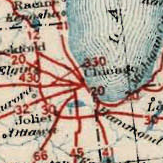
\includegraphics[width=\dimexpr.2\textwidth-8pt]{chicago} &
    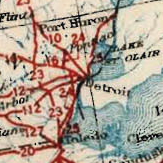
\includegraphics[width=\dimexpr.2\textwidth-8pt]{detroit} &
    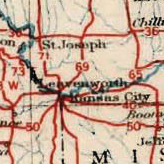
\includegraphics[width=\dimexpr.2\textwidth-8pt]{kansas-city} &
    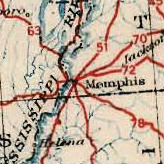
\includegraphics[width=\dimexpr.2\textwidth-8pt]{memphis} &
    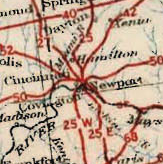
\includegraphics[width=\dimexpr.2\textwidth-8pt]{newport}  \\
  \end{tabular}
  \caption{Large cities have many direct routes to them. (Source:
  Map of the final U.S. Highway system as approved November 11, 1926.
  This map is in the public domain.)}
  \figlabel{us-map}
\end{figure}

\noindent
%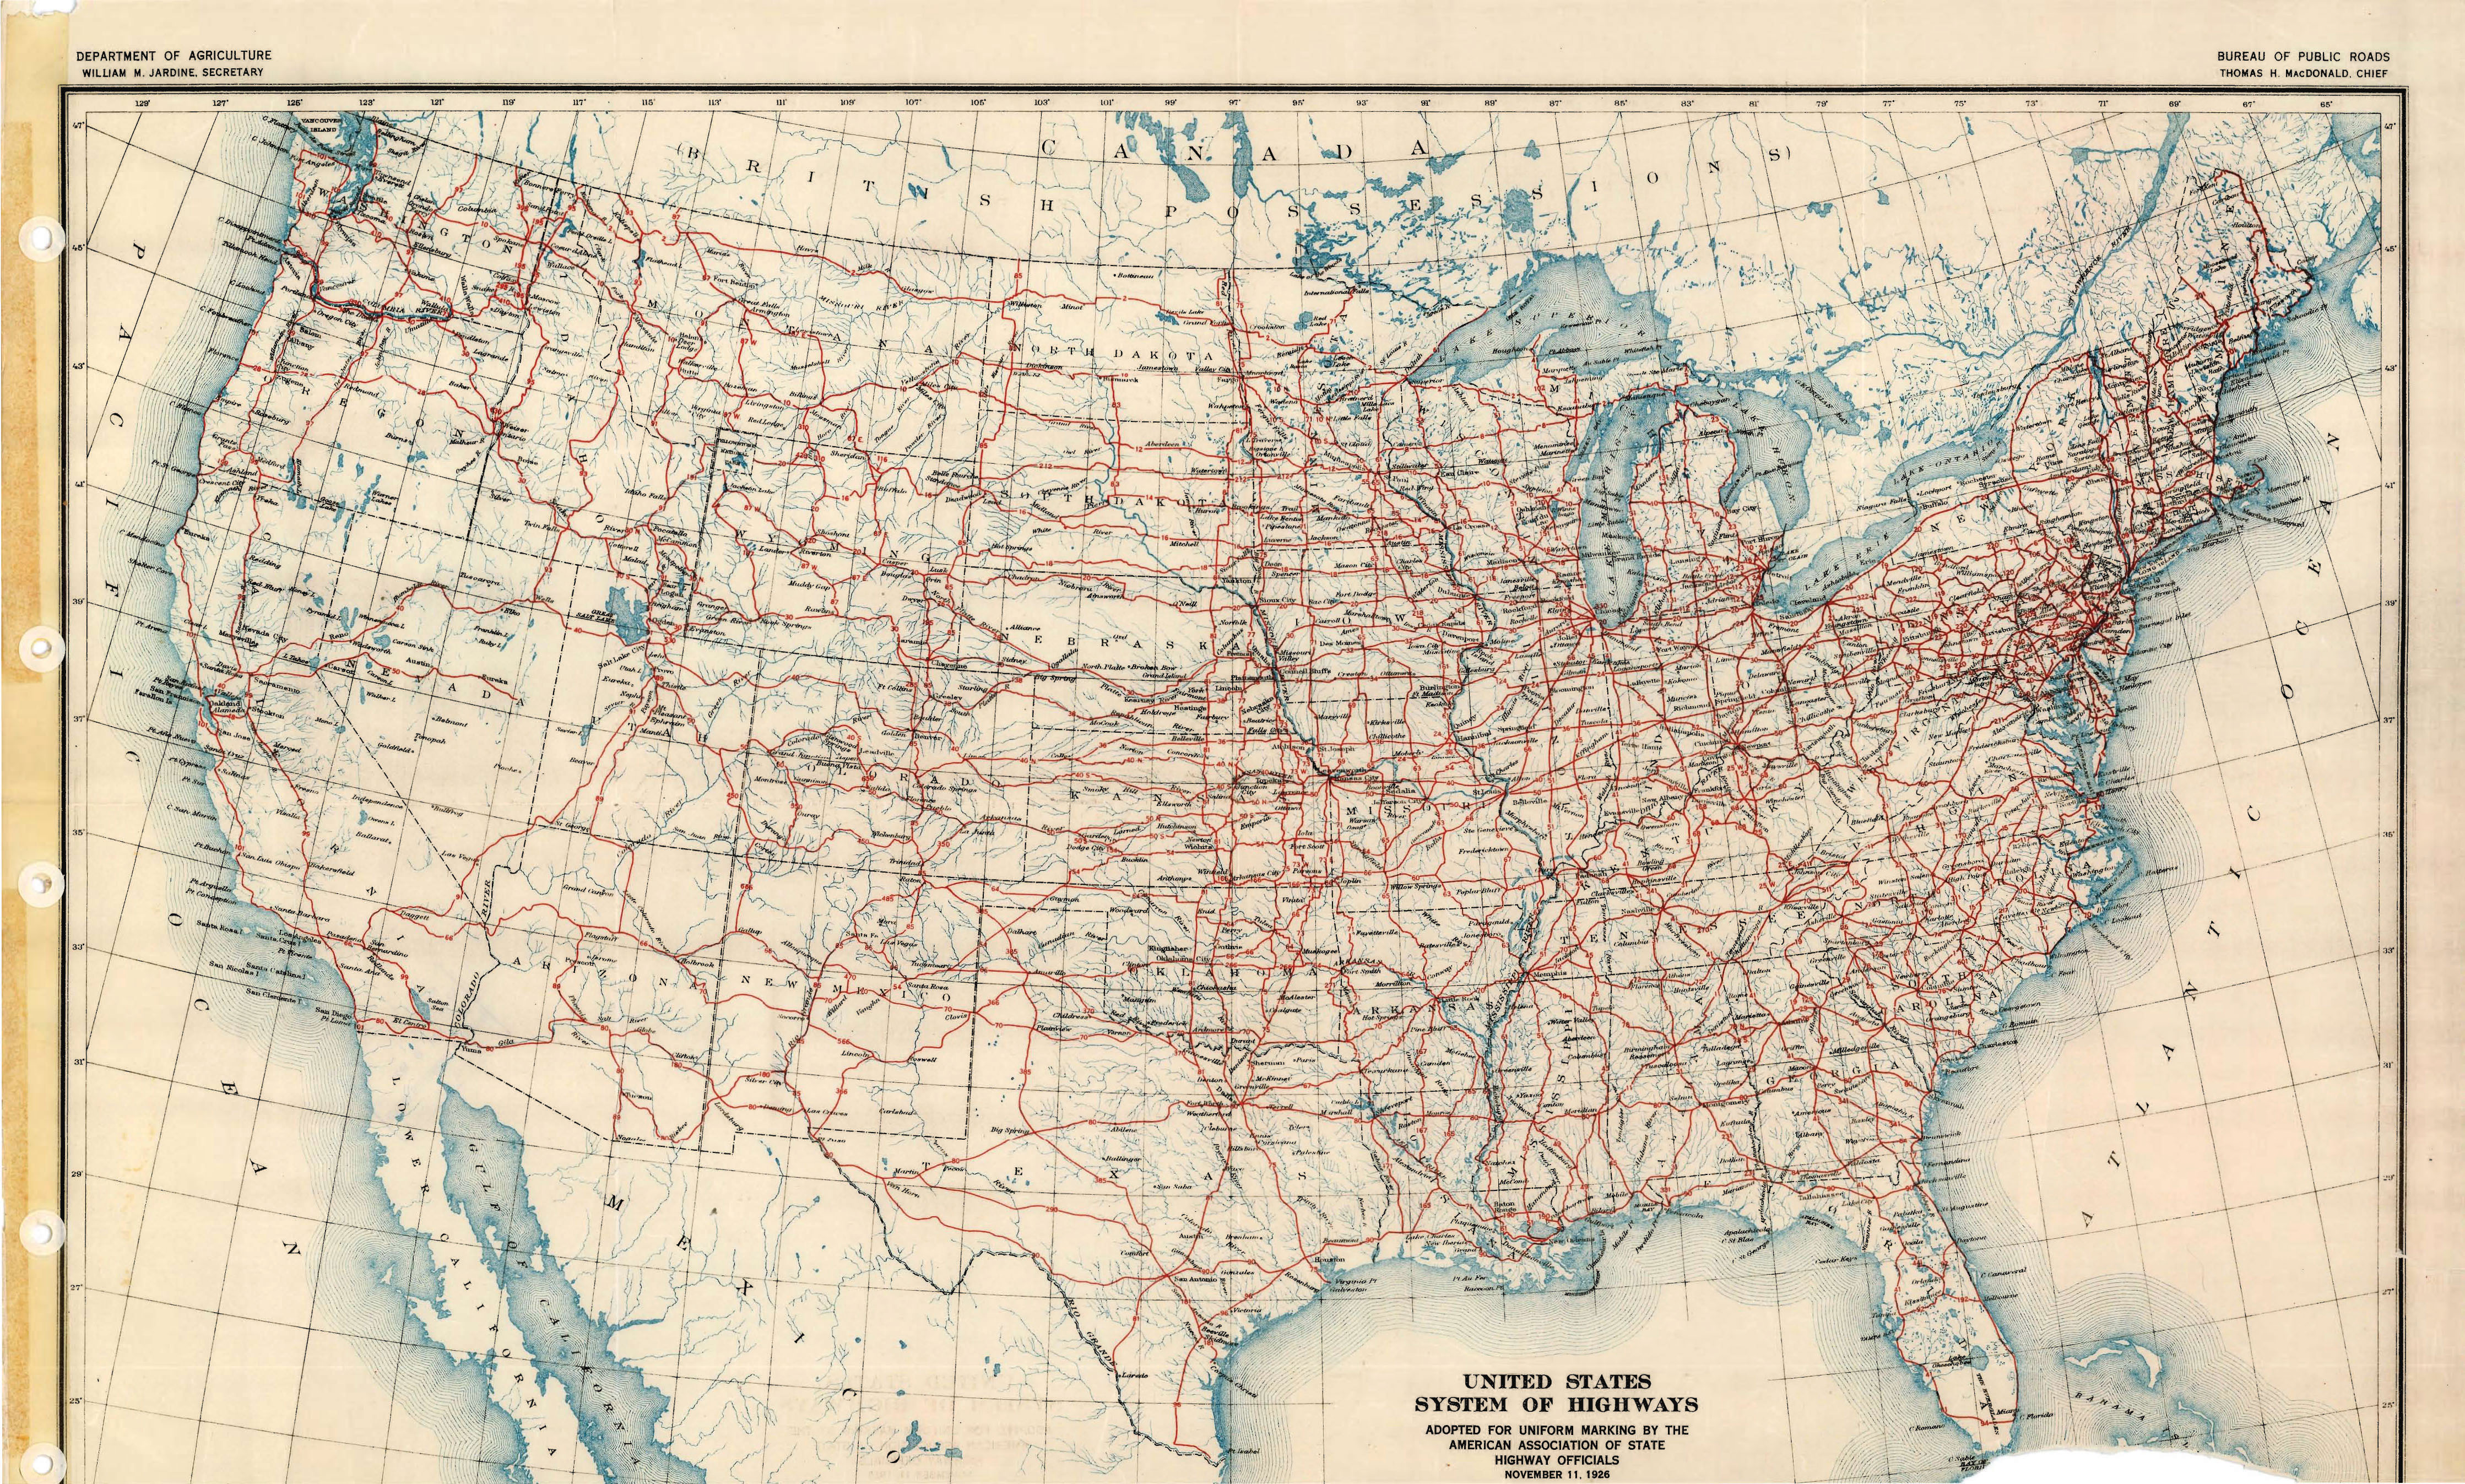
\includegraphics[totalwidth=0.48\textwidth,width=0.48\textwidth,trim=3in 3in 3in 3in, clip=true]{1926us.jpg}

\subsection{Open Problems}

Our results leave many areas open for further research.  We say that a
graph, $G=(V,E)$ has \emph{good average stretch} if $\asf(G)=1+o_n(1)$
and $|E|=O(n)$.

The following open problems have to do with strengthenings of
\thmref{upper-bound} in which $G$ has additional properties.

\begin{op}
  Given a point set, $V$, does there always exist a good average stretch
  graph $G=(V,E)$ whose total edge length is close to that of the minimum
  spanning tree?
\end{op}

\begin{op}
  Given a point set, $V$, does there always exist a good average stretch
  graph $G=(V,E)$ whose maximum degree is bounded by a constant?
\end{op}

\begin{op}
  Given a point set, $V$, does there always exist a good average stretch
  graph $G=(V,E)$ that is $k$-fault tolerant? That is, for any set
  $F\subset V$, $|F|\le k$, $\asf(G\setminus F)=1+o_n(1)$.
\end{op}

\begin{op}
  Bose \etal\ \cite{bose.dujmovic.ea:robust} define $f(k)$-robust spanners
  in terms of the (worst-case) stretch factor and their definition
  extends naturally to average stretch factor.  Given a point set, $V$,
  does there always exist a good average stretch graph $G=(V,E)$ that
  is $f(k)$-robust, for some reasonable function $f(k)$?
\end{op}


The following question asks if the upper-bound can be proven in a more
general setting:

\begin{op}\oplabel{metric-space}
  What conditions on a metric space $(V,d)$ are necessary and sufficient
  so that there always exist a graph $G=(V,E)$, $|E|\in O(n)$ with
  $\asf(G)=1+o_n(1)$?  (Here shortest paths in $G$ are measured in terms
  of the cost of their edges in the metric space.)
\end{op}

It seems likely that some of the techniques used to prove
\thmref{upper-bound} are applicable to metric spaces of bounded doubling
dimension \cite[Section~10.13]{heinonen:lectures}.  Is bounded doubling
dimension the weakest possible restriction on the metric space?  It is
clear that some restrictions on the metric space are required: In the
metric space in which all points have unit distance, the stretch factor
of a graph, $G=(V,E)$, having $m$ edges is at least
\[
    \binom{n}{2}^{-1}\left(m + 2\left(\binom{n}{2}-m\right)\right) 
\]
since, if there is no edge between $u$ and $w$ in $G$, then $\|uw\|_G
\ge 2$.  Therefore any graph with average stretch factor $1+o_n(1)$
must have $\binom{n}{2}-o(n^2)$ edges.

\section*{Acknowledgement}

The authors of this paper are partly funded by NSERC and CFI.

\bibliographystyle{abbrvurl}
\bibliography{avgstretch}

\newpage

\begin{titlepage}
\appendix
\section{Full Version}
\hspace{.3\textheight}
\begin{center}
 \Huge
 This page separates the extended abstract from the full version.
\end{center}
\end{titlepage}

\end{document}


